After investigating the throughput of the blockchain, we also tested our
Peer-2-Peer network and capability to deal with different block confirmation
times. As a reminder, the technology tested here is capable of changing
different blockchain parameters on the fly. One of this parameters is the block
confirmation time which represents the time between the blocks in our
synchronous consensus mechanism delegated proof-of-stake (DPOS).

\begin{figure}[!htp]
 \centering
 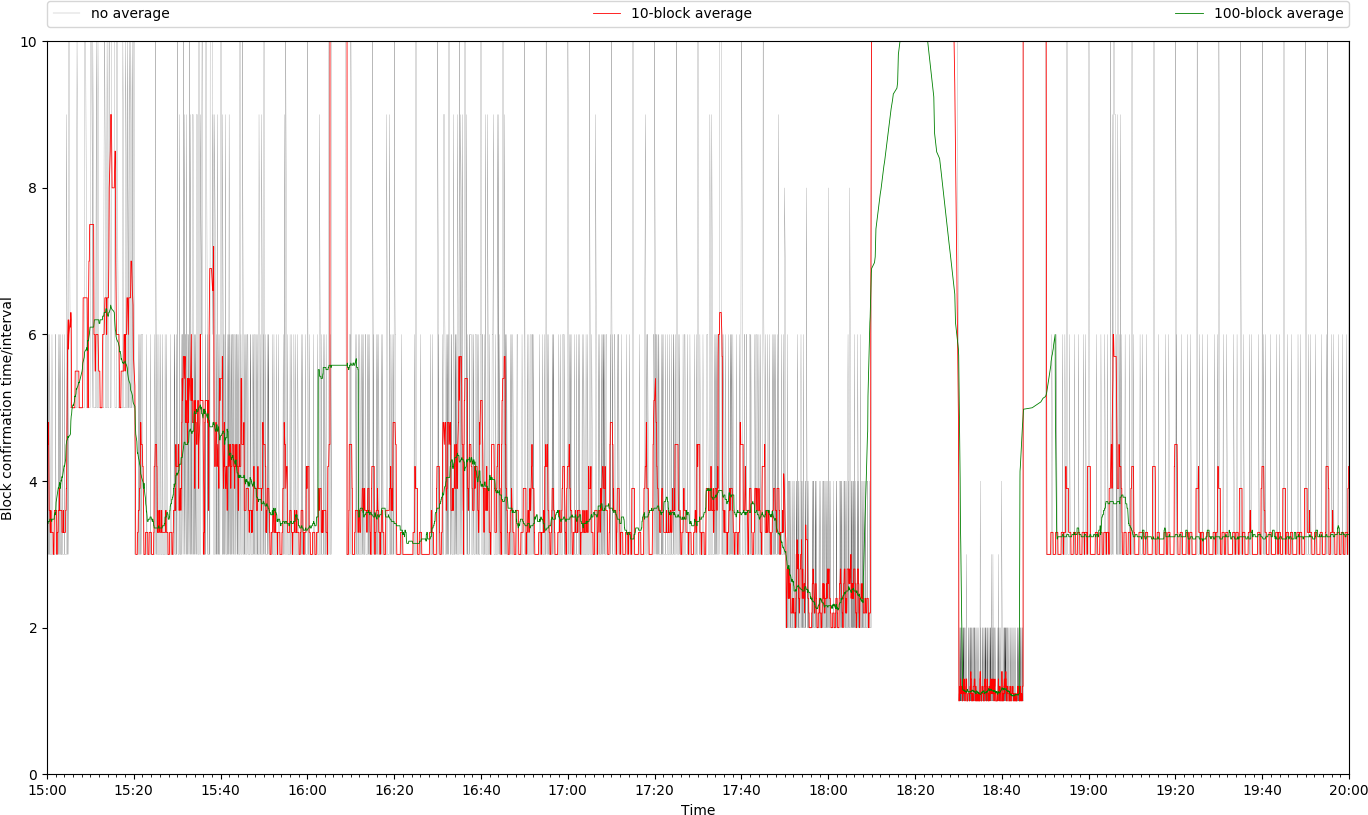
\includegraphics[width=\linewidth]{figures/stress-test-block-time-full.png}
 \caption{Max ops/s during the stress-test}
 \label{fig:time-full}
\end{figure}

In \cref{fig:time-full}, we can see the actual block confirmation time as
tracked by the blockchain. These numbers have been obtained from each block
header that also contains the time stamp. Little variations are to be expected
due to slightly inaccurate synchronization of the local time, while large
deviations indicate one or multiple validators to have missed their blocks. The
graphs shown in the figure are average over \SI{100}{blocks} to reduce the
noise in the figure.

We can see that, during the stress-test, multiple different block confirmation
times have been tested, starting with \SI{5}{s}, going down to \SI{2}{s}, then
up to \SI{10}{s} until we decided to also test \SI{1}{s} block confirmation
times. Unfortunately, we have seen some witnesses not produce during large
parts of the stress-test which is why the averages are above the target rates
most of the time. For our next stress-test we plan to be more strict in
replacing witnesses when they miss to produce blocks.

\begin{figure}[!htp]
 \centering
 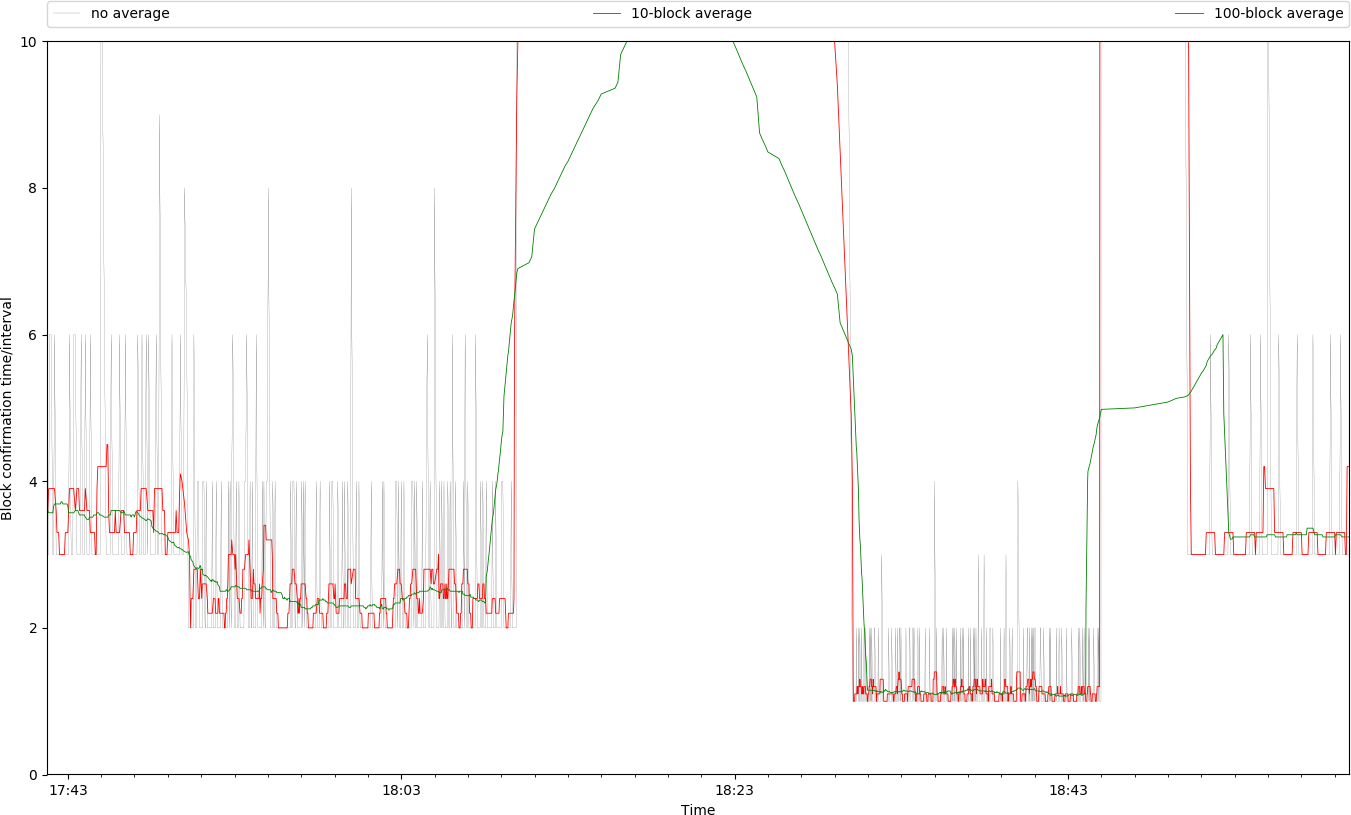
\includegraphics[width=\linewidth]{figures/stress-test-block-time-1sec.png}
 \caption{Max ops/s during the stress-test}
 \label{fig:time-1se}
\end{figure}

In \cref{fig:time-1sec} we have zoomed into the period where we have reduced
the confirmation time to \SI{1}{s}. We can see that most of the blocks have
been produce in time with only up to 3 validators not having produced in time
(i.e. the black peaks going up to at most \SI{4}{s}). This came as a big
surprise to us as we have expected a higher block-miss rate all together.
